\documentclass[12pt,compress,ngerman,utf8,t,usenames,dvipsnames]{beamer}
\usepackage[ngerman]{babel}


\title{Hi-C interaction matrix correction using ICE in Rust}
\subtitle{Bachelor thesis defense}
\author{Felix Karg}


\graphicspath{ {../template/} {./graphics/} } % add further graphics paths here



\usepackage{etex}
\usepackage{graphicx}
\usepackage[export]{adjustbox}
\usepackage{multicol}
\usepackage{pdfpcnotes}
\usepackage{pdfpages}
% \usepackage[dvipsnames]{xcolor}


% \usepackage{minted}
% \usemintedstyle{pastie}


\usetheme[numbering=fraction, progressbar=frametitle]{metropolis}


\date{December 29, 2020}
% \date{12. Juli 2019}


% \institute{Add Your Institute here}
% \titlegraphic{\vspace{4cm} \hspace{7cm} \includegraphics[height=2cm]{Logo_INST}}
% \titlegraphic{\vspace{4cm} \hspace{7cm} \Huge\LaTeX}

\iftwocols
\AtBeginSection[]
{
    \large
    \begin{frame}{Agenda}
        \begin{multicols}{2}
            \tableofcontents[currentsection]
        \end{multicols}
        \clearpage
    \end{frame}
}

\AtBeginSubsection[]
{
    \large
    \begin{frame}{Agenda}
        \begin{multicols}{2}
            \tableofcontents[currentsection,currentsubsection]
        \end{multicols}
        \clearpage
    \end{frame}
}

\else

\AtBeginSection[]
{
    \large
    \begin{frame}{Agenda}
        \tableofcontents[currentsection]
        \clearpage
    \end{frame}
}

\AtBeginSubsection[]
{
    \large
    \begin{frame}{Agenda}
        \tableofcontents[currentsection,currentsubsection]
        \clearpage
    \end{frame}
}
\fi


\begin{document}

\maketitle

% multicols from:
% https://tex.stackexchange.com/questions/24343/splitting-toc-into-two-columns-on-single-frame-in-beamer

%%%%%%%%%%%%%%%%%%%%%%%%%%%%%%%%%%%%%%%%%%%%%%%%%%%%%%%%%%%%%%%%%%%%%%%%%%%%%%%%%%%%%%%%%%%%%%%%%%%%%%%%%%%%%%%%%%%

\iftwocols
\begin{frame}{Agenda}
    \large
    \begin{multicols}{2}
%        \tableofcontents[hidesubsections]
        \tableofcontents[]
    \end{multicols}
    % \clearpage
\end{frame}

\else

\begin{frame}{Agenda}
    \large
%   \tableofcontents[hidesubsections]
    \tableofcontents[]
    % \clearpage
\end{frame}
\fi


\newcommand{\code}[1]{
    \begin{center}
    \setlength{\fboxrule}{1pt}
    \setlength{\fboxsep}{8pt}
        {\fbox{\parbox{0.81\textwidth}{#1}}}
   \end{center}
}

\newenvironment{codeboxed}[1]
        {\begin{minipage}{\linewidth}\begin{center}#1\\[1ex]\begin{tabular}{|p{\textwidth}|}\hline}
        {\\\hline\end{tabular}\end{center}\end{minipage}}


\newcommand{\backupbegin}{
   \newcounter{finalframe}
   \setcounter{finalframe}{\value{framenumber}}
}

\newcommand{\backupend}{
   \setcounter{framenumber}{\value{finalframe}}
}


\newcommand{\mailto}[1]{
    \href{mailto:#1}{#1}
}

\newcommand{\todo}[1]{
    {\Large\color{red}{(TODO: #1)}}
}

% \definecolor{green1}{RGB}{38, 69, 37} % #264525
\definecolor{green1}{RGB}{72, 129, 69} % #488145
% \definecolor{blue1}{RGB}{7, 43, 94} % #072b5e
\definecolor{blue1}{RGB}{14, 82, 179} % #0e52b3
% \definecolor{violet1}{RGB}{58, 38, 68} % #3a2644
\definecolor{violet1}{RGB}{108, 72, 126} % #6c487e
% \definecolor{orang1}{RGB}{, , 0} % #663400
\definecolor{orang1}{RGB}{193, 98, 0} % #c16200


\newcommand{\green}[1]{
    \textcolor{green1}{#1}
}
\newcommand{\blue}[1]{
    \textcolor{blue1}{#1}
}
\newcommand{\vio}[1]{
    \textcolor{violet1}{#1}
}
\newcommand{\orang}[1]{
    \textcolor{orang1}{#1}
}




\newif\ifonline
\onlinefalse
% \onlinefalse


%%%%%%%%%%%%%%%%%%%%%%%%%%%%%%%%%%%%%%%%%%%%%%%%%%BEGINNING%%%%%%%%%%%%%%%%%%%%%%%%%%%%%%%%%%%%%%%%
\section{Examples}

\begin{frame}[c]
     Here a citation: \cite{benchcpp}
\end{frame}

\begin{frame}[c]{Example slide}
    \Large
    \begin{itemize}[<+->]
        \item First Element
        \item Second Element
        \item Third Element
    \end{itemize}
\end{frame}

\begin{frame}[c]{Other example slide}
    \Large
    \begin{itemize}[<+(1)->]
        \item First Element
        \item Second Element
        \item Third Element
    \end{itemize}
\end{frame}

\begin{frame}[c]{Yet another example slide}
    \Large
    \begin{itemize}
        \item First Element
            \pause
        \item Second Element
            \pause
        \item Third Element
    \end{itemize}
\end{frame}










\begin{frame}{Content}
    \large
%     \begin{multicols}{2}
%         \tableofcontents[hidesubsections]
        \tableofcontents[]
%     \end{multicols}
    % \clearpage
\end{frame}



% \input{chapters/motivation}
\section{Hi-C}

\begin{frame}[c]{High-Throughput 3C (Hi-C)}
    \normalsize
    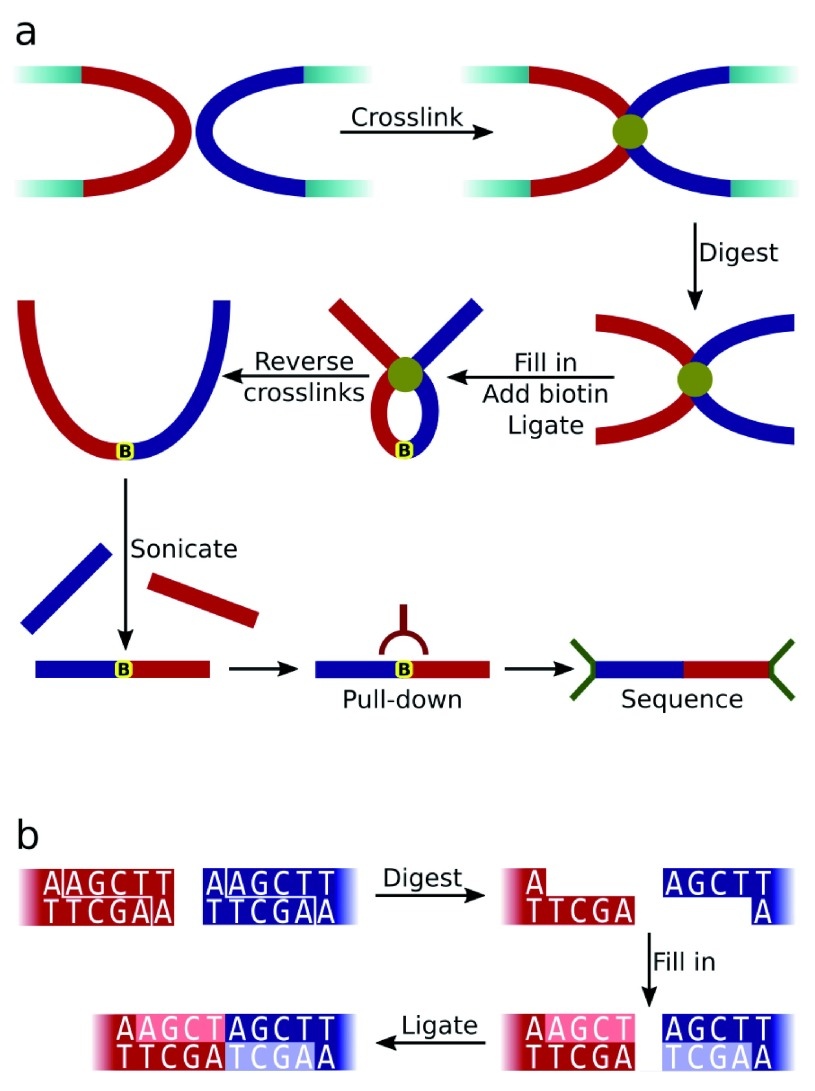
\includegraphics[scale=2.4, trim=0 40 0 6, clip]{f1000research-4-7903-g0000} \\
    Image adapted from \cite{wingett2015hicup}.
\end{frame}

\begin{frame}[c]{High-Throughput 3C (Hi-C)}
    Several biases:
    \begin{itemize}[<+(1)->]
        \item Some regions are easier labeled with biotin than others
        \item PCR artifacts \cite{wingett2015hicup}
        \item Sequencing itself has multiple biases \cite{aird2011analyzing}
        \item Where to map multiple/unclear reads
    \end{itemize}
    % \only<2>{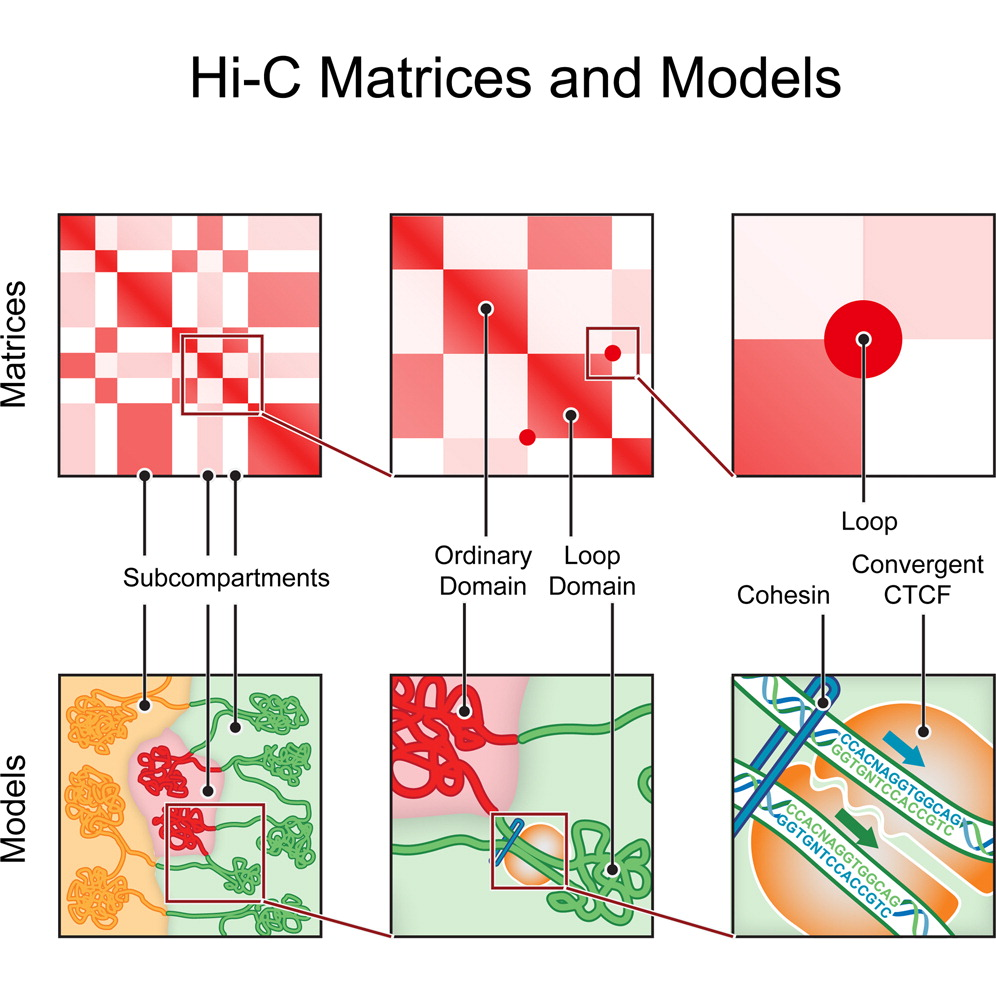
\includegraphics[scale=1.5, trim=0 0 82 130,clip]{HiCMatricesModels} \\
    % Image adapted from \cite{rao20143d}.}
    % Biases for each step:
    %
    % - Some regions do easier biotin labeling than others
    % - PCR artifacts are included
    % - Sequencing itself has multiple biases
    % - Where to map multiple/unclear reads ?
    % - differing chromatin states
    % - more ...

\end{frame}

% \begin{frame}[c]% {Chromosome Conformation Technologies}
%     \normalsize
%     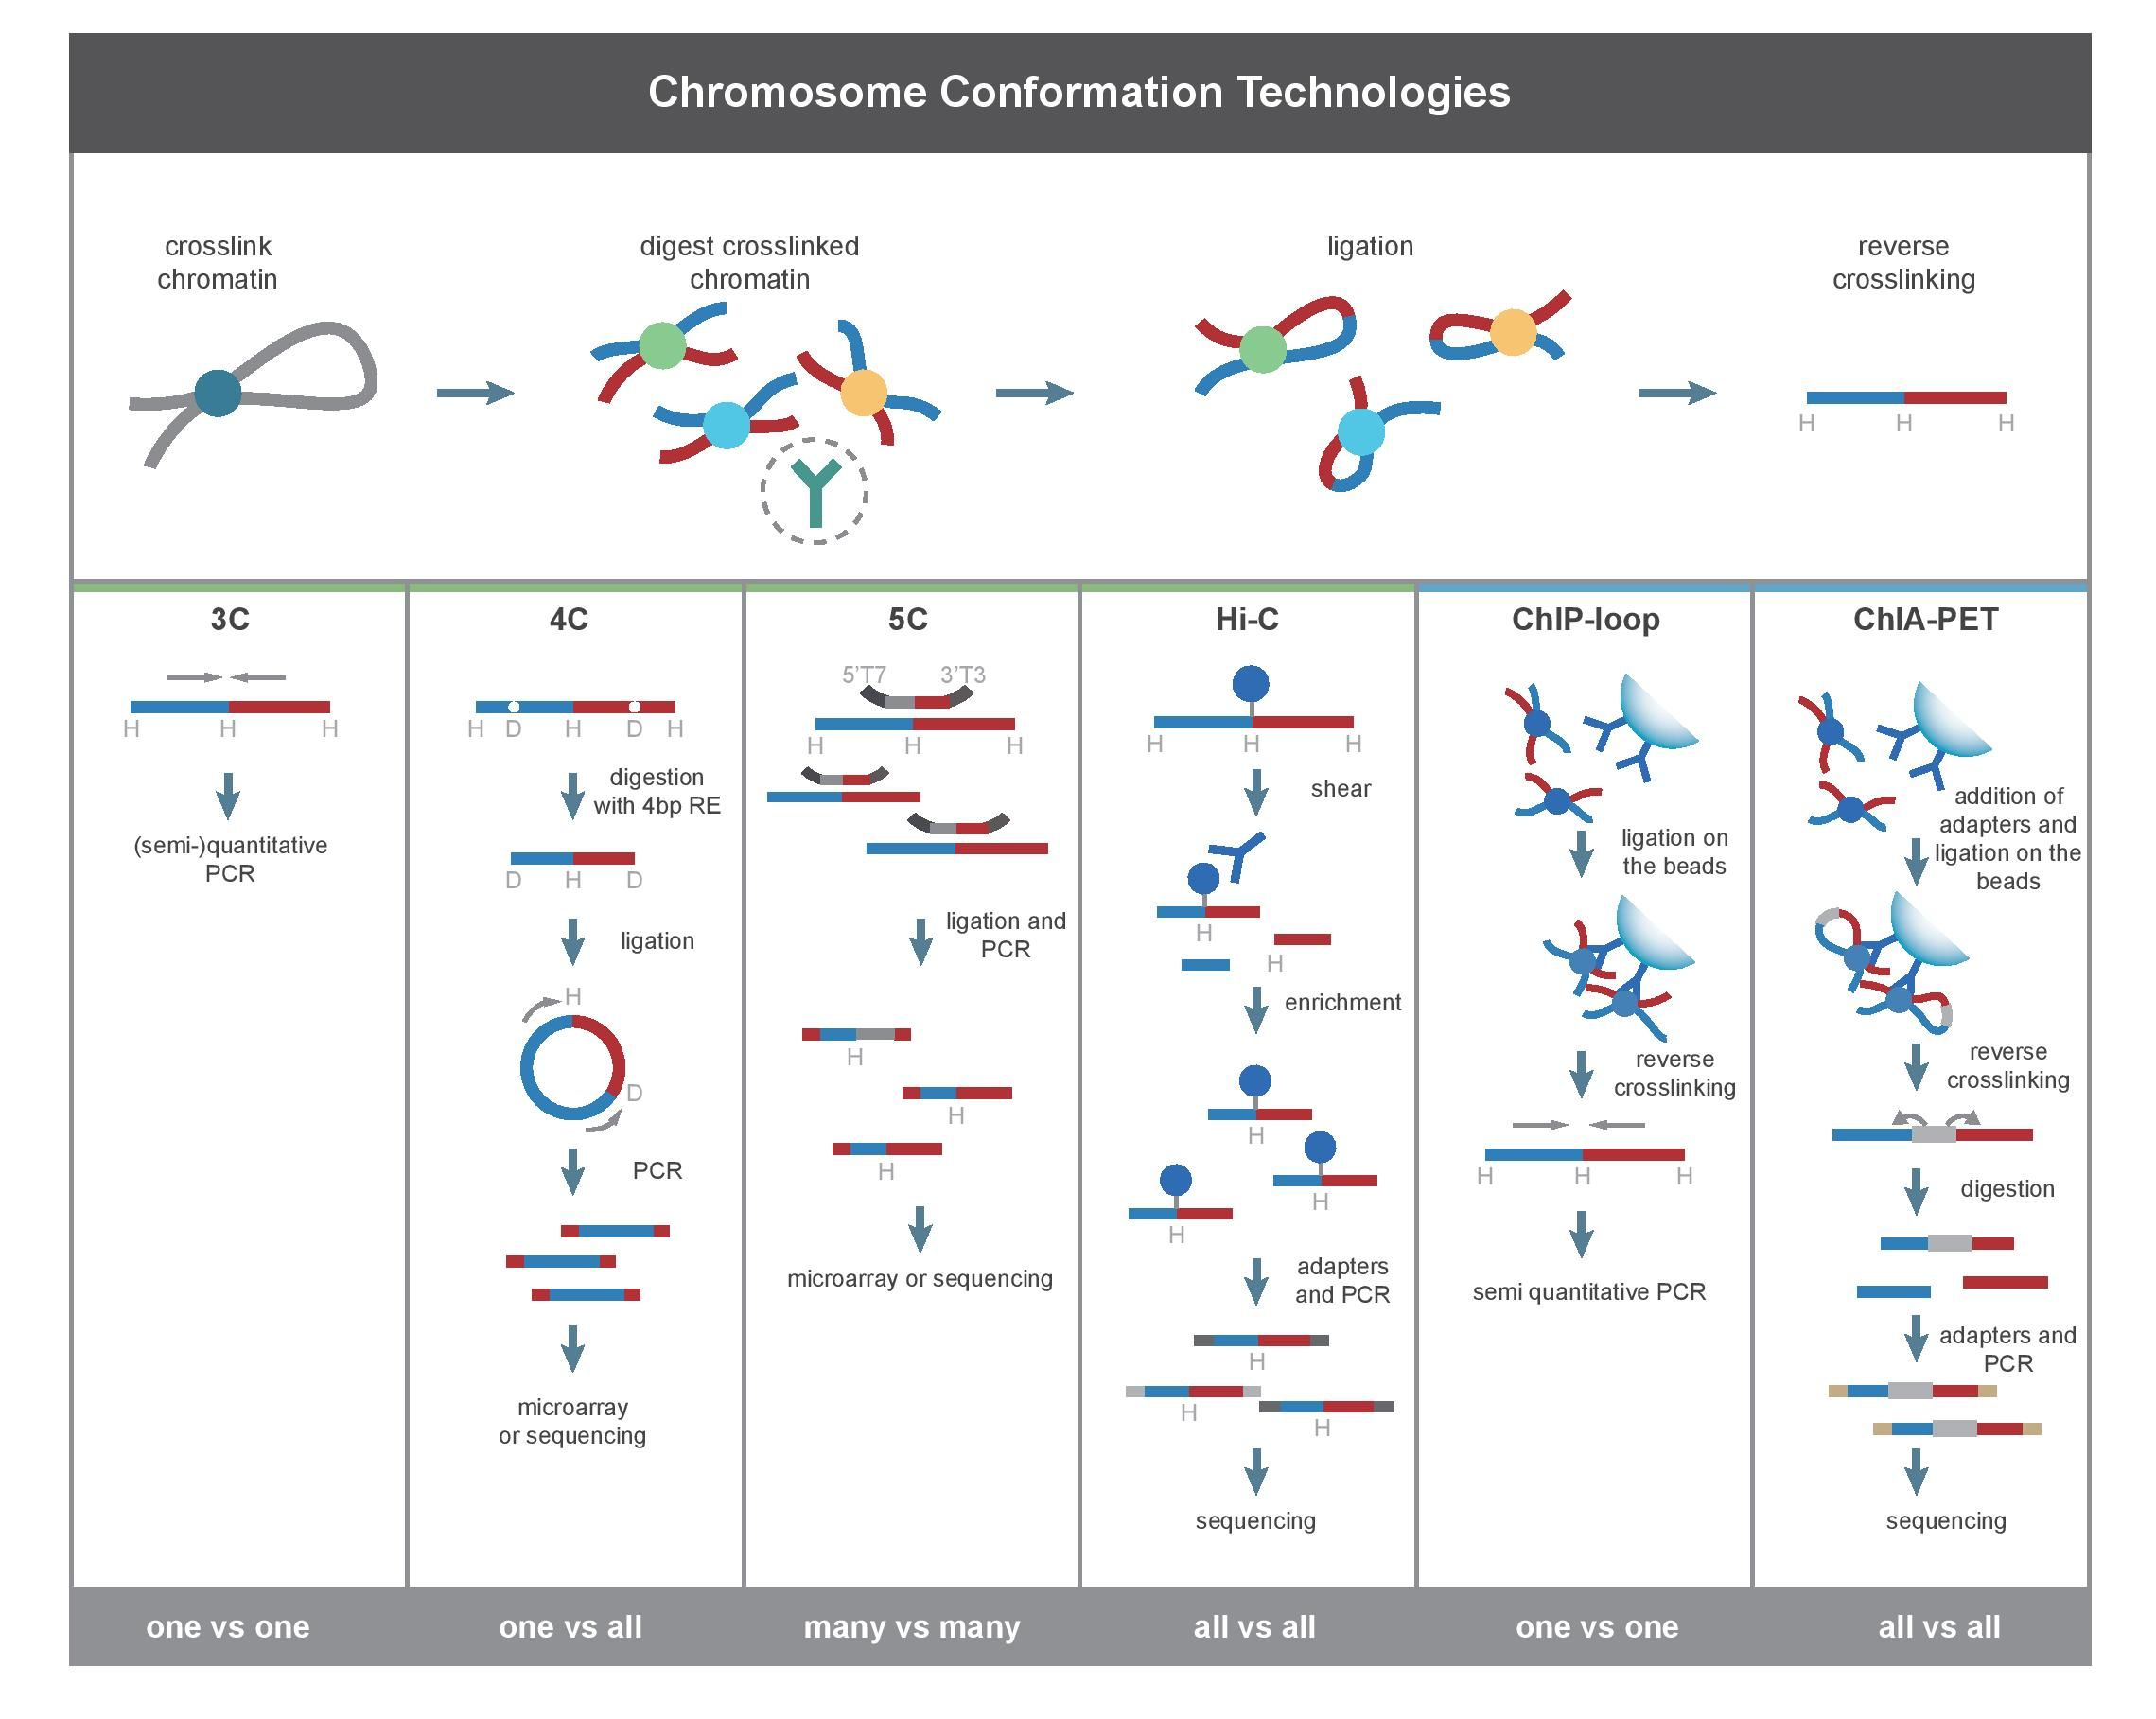
\includegraphics[scale=0.55]{Chromosome_conformation_techniques} \\
%     Image from \cite{Li2014}.
% \end{frame}


% Make introduction of Hi-C with focus to potential biases


\begin{frame}[c]{HiCExplorer}
    \large
    Helpful tools, especially for:
    \begin{itemize}[<+(1)->]
        \item Data correction
        \item Analysis
        \item Visualization
    \end{itemize}
\end{frame}


% \begin{frame}[c]{HiCExplorer}
%     \normalsize
%     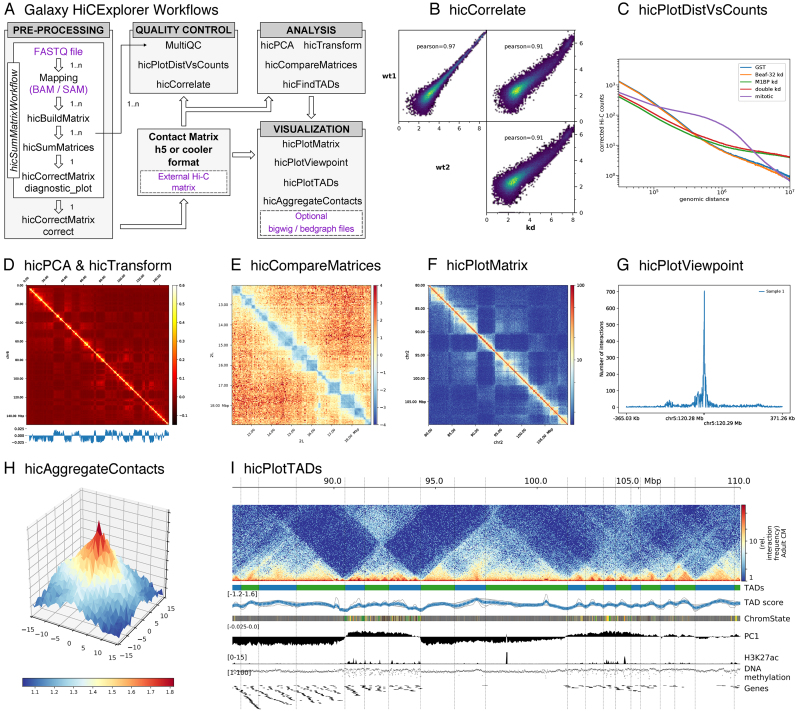
\includegraphics[scale=2.5,trim=37 0 0 45,clip]{HiCExplorer} \\
%     Image adapted from \cite{wolff2018galaxy}.
% \end{frame}



\section{ICE}

\begin{frame}[c]{Iterative Correction and Eigenvector decomposition}
    \Large
    Algorithm as described in \cite{imakaev2012iterative}.
\end{frame}


\begin{frame}[c]{Iterative Correction and Eigenvector decomposition}
    \Large
    \begin{itemize}% [<+(1)->]
        \item<2-> $O_{ij}$: raw data
        \item<6-> $S_i$: sum of row $i$ of $W_{ij}$
        \item<5-> $B_i, B_j$: cumulative biases
        \item<3-> $T_{ij}$: relative contact probabilities
        \item<4-> $W_{ij}$: working copy of $O_{ij}$, becoming $T_{ij}$
    \end{itemize}
\end{frame}

\begin{frame}[c]{Iterative Correction and Eigenvector decomposition}
    \Large
    Goal: Obtain $B$ and $T_{ij}$. \\ \pause Do this by explicitly solving:
    \begin{equation} \label{eq:1}
    O_{ij} = B_i B_j T_{ij}
    \end{equation}
    \begin{equation} \label{eq:2}
    \sum^N_{i=1, |i-j|>1} T_{ij} = 1
    \end{equation}
\end{frame}


\begin{frame}[c]{Iterative Correction and Eigenvector decomposition}
    \begin{equation}
    \forall_j\sum^N_{i=1}T_{ij} = 1
    \end{equation}
    \begin{equation}
        \forall_i\sum^N_{j=1}T_{ij} = 1
    \end{equation}
\end{frame}

\begin{frame}[c]{Iterative Correction and Eigenvector decomposition}
    \Large
    Each iteration, solve:
    \pause
    \onslide<2->{
    \begin{equation}\label{eq:3}
        S_i = \sum_j W_{ij}
    \end{equation}
    \begin{equation}\label{eq:4}
        \Delta B_i = S_i / mean(S)
    \end{equation}
    }
    \vspace*{-\baselineskip}
    \onslide<3>{
    \begin{equation}\label{eq:5}
        W_{ij} = W_{ij} / \Delta B_i \Delta B_j
    \end{equation}
    \begin{equation}\label{eq:6}
        B_i = B_i \cdot \Delta B_i
    \end{equation}
    }
\end{frame}

% Introduce the ICE algorithms based on graphics / Formulas







% \section{Current Implementations}


% make nice flow-graphs about pre-processing, iterating and comparing

\section{Rust}


\begin{frame}[c]{Rust: Short History}
    \Large
    \begin{itemize}[<+(1)->]
        \item Started out in 2006
        \item Mozilla started sponsoring in 2009
        \item Self-compiled in 2011
        \item 1.0 released in 2015
    \end{itemize}
\end{frame}

\begin{frame}[c]{Rust: Language Features}
    \Large
    \begin{itemize}[<+(1)->]
        \item Syntax seems similar to C/C++
        \item Semantically closer to ML/Haskell
        \item Memory-Safety (no NULL)
        \item Memory Management (RAII)
        \item Ownership
        \item Borrowing
        \item Lifetimes
    \end{itemize}
\end{frame}




\begin{frame}[c]{Rust: Comparison}
    \normalsize
    \vfill
    \begin{tabular}{lrrr}
        \textbf{Speed coparison} & C & Rust & C++ \\ \hline
        n-body & 7.49 & \textbf{5.72} & 8.18 \\
        binary-trees & 3.48 & \textbf{3.15} & 3.79 \\
        pidigits & \textbf{1.75} & \textbf{1.75} & 1.89 \\
        reverse-complement & 1.78 & 1.61 & \textbf{1.55} \\
        spectral-norm & 1.98 & \textbf{1.97} & 1.98 \\
        fannkuch-redux & \textbf{8.61} & 10.23 & 10.08 \\
        k-nucleotide & 5.01 & 5.25 & \textbf{3.76} \\
        fasta & 1.36 & 1.47 & \textbf{1.33} \\
        mandelbrot & 1.65 & 1.96 & \textbf{1.50} \\
        regex-redux & \textbf{1.46} & 2.43 & 1.82 \\ \hline
        Fastest in: & 3/10 & 4/10 & 4/10 \\
    \end{tabular} \\ \\
    \footnotesize
    Runtime measured in \textbf{seconds}. Numbers for C from \cite{benchc} and for C++ from
    \cite{benchcpp}. Both show the same numbers for Rust.

\end{frame}



\begin{frame}[c]{Rust: Advantages and Disadvantages}
    General Advantages:
    \begin{itemize}[<+(1)->]
        \item High-Level Features
        \item Fast Language
        \item Safe Memory handling
        \item Strong Type system
    \end{itemize}
    \pause
    General Disadvantages:
    \begin{itemize}[<+(1)->]
        \item Young ecosystem
        \item Steep learning curve
        \item Higher initial compile times
        \item Language Features not yet available
    \end{itemize}
\end{frame}


\begin{frame}[c]{Rust: Advantages and Disadvantages}
    Advantages for this Project:
    \begin{itemize}[<+(1)->]
        \item Own CSRMatrix implementation
        \item No big dependencies
        \item Faster and smaller, very specific
    \end{itemize}
    \pause
    Disadvantages for this Project:
    \begin{itemize}[<+(1)->]
        \item No general implementation of CSRMatrix
        \item Only subset of features when compared to SciPy implementation
    \end{itemize}
\end{frame}




\section{Integration of Rust in Python}


\begin{frame}[c]{API: Rust to Python}
    There are three main ways to use Rust from Python:
    \pause
    \begin{itemize}[<+->]
        \item rust-cpython
        \item pyO3
        \item dylib
    \end{itemize}
\end{frame}

\begin{frame}[c]{rust-cpython}
    \begin{itemize}[<+(1)->]
        \item Similar to C-Python headers
        \item Grants access to the Python GIL
        \item Renaming needed
        \item Stable Rust
        \item Easy package creation
    \end{itemize}
\end{frame}


\begin{frame}[c]{pyO3}
    \begin{itemize}[<+(1)->]
        \item Fork from rust-cpython
        \item Grants access to the Python GIL
        \item Renaming needed
        \item Nightly Rust
        \item Easy package creation
    \end{itemize}
\end{frame}


\begin{frame}[c]{dylib}
    \begin{itemize}[<+(1)->]
        \item Recommended in the Rust book
        \item No renaming needed
        \item Stable Rust
        \item No access to the Python GIL
        \item Package creation possible
    \end{itemize}
\end{frame}



\begin{frame}[c]{API Comparison for Rust in Python}
    \normalsize

\begin{tabular}{@{}lrrr@{}}
    \textbf{API Comparison} & rust-cpython & pyO3 & dylib \\
    \hline
    Memory from Python              & Yes           & Yes & \textbf{Optional} \\
    Renaming needed                 & Yes           & Yes & \textbf{No} \\
    Stable Rust                     & \textbf{Yes}  & No  & \textbf{Yes} \\
    Platform-specific               & Yes           & Yes & \textbf{No} \\
    Implementation effort           & Medium        & Medium & \textbf{Low} \\
    Creating python packages        & \textbf{Easy} & \textbf{Easy} & Normal \\ \\
    \hline
    Good in: & 2/6 & 1/6 & \textbf{5/6} \\
\end{tabular}
\end{frame}









\section{Results}


\begin{frame}[c]{Compared implementations}
    \begin{itemize}[<+(1)->]
        \item 'ICE' - Python implementation
        \item 'KR' - C++ implementation
        \item 'RUST' - this implementation
    \end{itemize}
\end{frame}



\begin{frame}[c,fragile]{Data for Testing}
    \normalsize
    \begin{tabular}{@{}lrr@{}}
        % \textbf{Matrix Details} & & & \\
        \textbf{Name}       & 25kb          & 50kb \\
        \hline
        Filesize            & 1.1 GByte     & 0.73 GByte     \\
        Size                & \verb|123,841|       & \verb|61,928| \\
        Bin length          & \verb|25,000|        & \verb|50,000| \\
        Non-zero elements   & \verb|1,530,533,003| & \verb|1,053,216,825| \\
    \end{tabular}
    % Data from \cite{rao20143d}.
\end{frame}




\begin{frame}[c]{Memory Requirements during correction}
    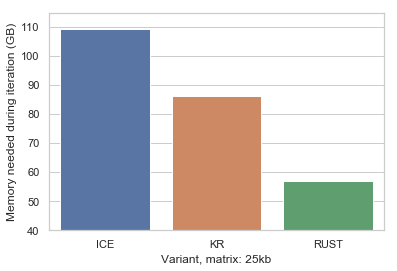
\includegraphics[scale=0.8]{memiter_25}
\end{frame}


\begin{frame}[c]{Peak Memory Usage}
    \only<1>{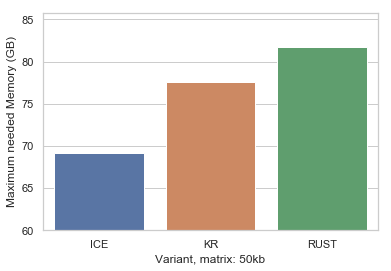
\includegraphics[scale=0.8]{maxresident_50}}
    \only<2>{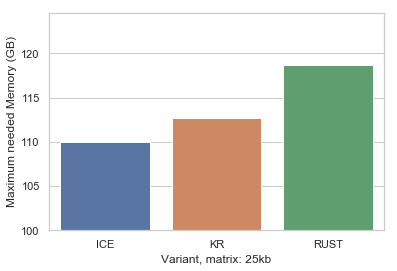
\includegraphics[scale=0.8]{maxresident_25}}
    \only<3>{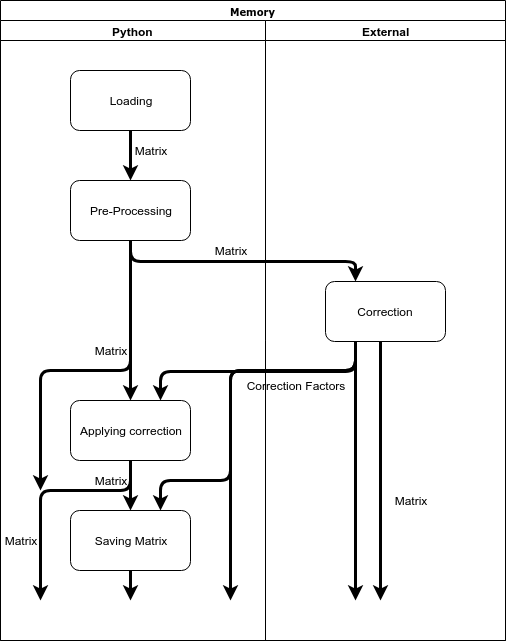
\includegraphics[scale=0.35]{correction_process}}
\end{frame}

\begin{frame}[c]{Comparison of Memory needs}
    \begin{tabular}{lrrr}
        \textbf{Memory needs Comparison} & ICE & KR & RUST \\
        \hline
        During correction (50kb) &   54.6 & 43.1 & \textbf{39.0}   \\
        Maximum          (50kb) &   \textbf{69.2} & 77.6 & 81.7 \\
        During correction (25kb) &   110.0 & 86.0 & \textbf{57.0}  \\
        Maximum          (25kb) &   \textbf{110.0} & 112.7 & 118.6 \\
    \end{tabular}
\end{frame}


% \begin{frame}[c]{Loading Times}
%     \only<2>{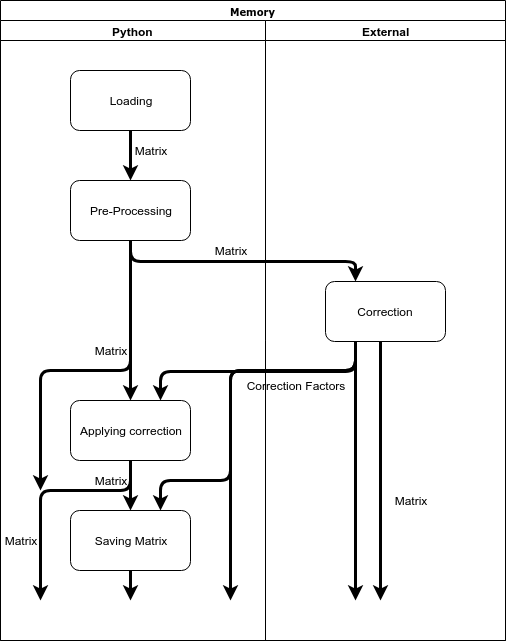
\includegraphics[scale=0.35]{correction_process}}
%     \only<3>{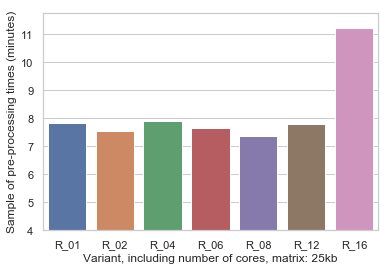
\includegraphics[scale=0.8]{loadtimes_25}}
%     \only<4>{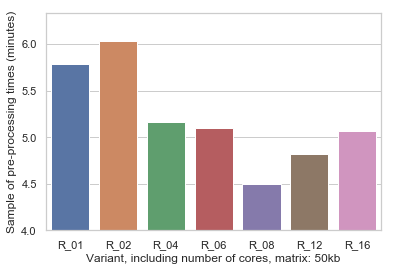
\includegraphics[scale=0.8]{loadtimes_50}}
% \end{frame}


\begin{frame}[c]{Runtime Length}
    \only<2>{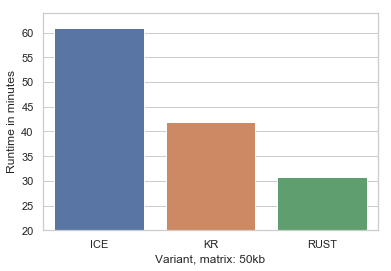
\includegraphics[scale=0.8]{runtime_50}}
    \only<3>{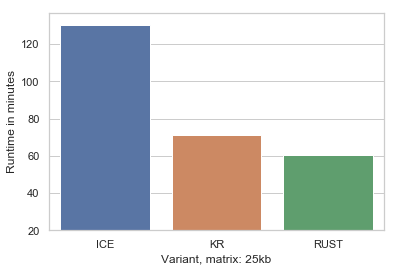
\includegraphics[scale=0.8]{runtime_25}}
\end{frame}


\begin{frame}[c]{Control Flow Diagram}
    \pause
    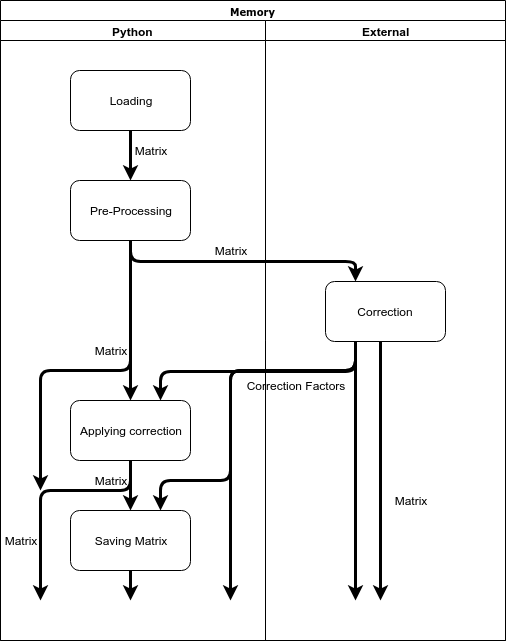
\includegraphics[scale=0.35]{correction_process}
\end{frame}


\begin{frame}[c]{Multicore Runtime Length Comparison}
    % \only<2>{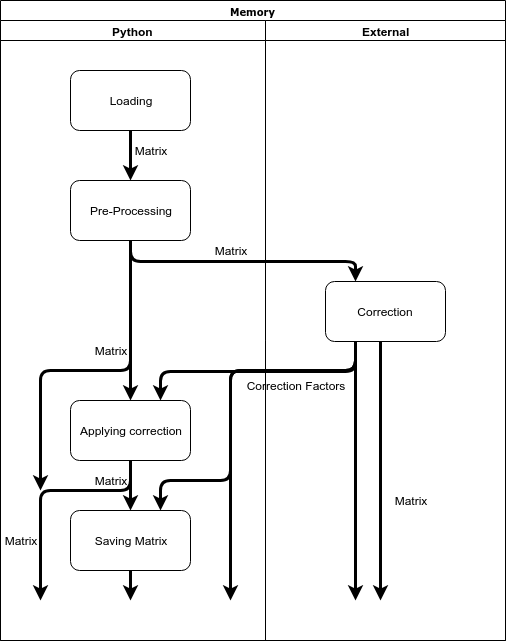
\includegraphics[scale=0.35]{correction_process}}
    \only<2>{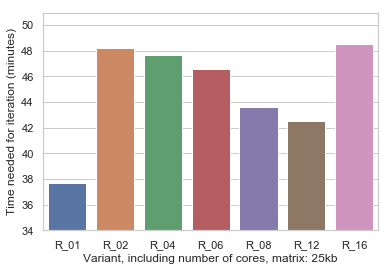
\includegraphics[scale=0.8]{compute_multi_25}}
    \only<3>{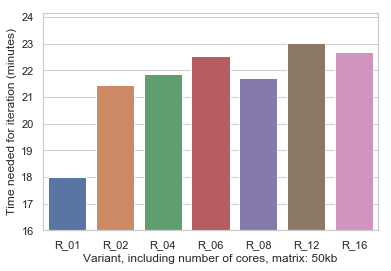
\includegraphics[scale=0.8]{runtime_multi_50}}
\end{frame}

\begin{frame}[c]{Overall Runtime Length Comparison}
    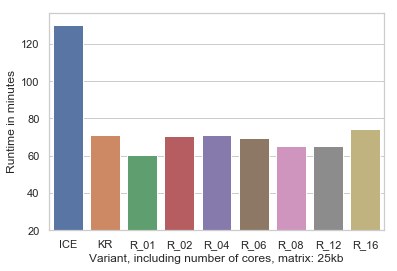
\includegraphics[scale=0.8]{runtime_multi_25}
\end{frame}

\begin{frame}[c]{Multicore Memory Comparison}
    \only<2>{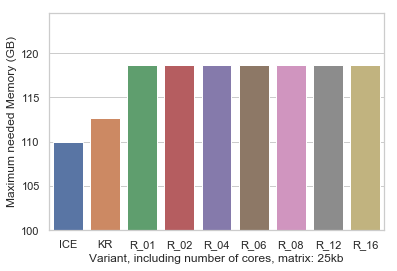
\includegraphics[scale=0.8]{maxresident_multi_25}}
    \only<3>{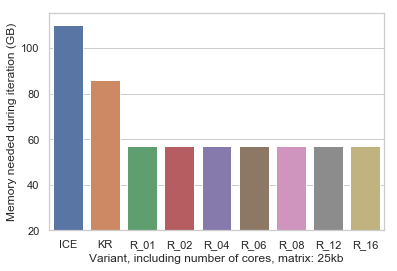
\includegraphics[scale=0.8]{memiter_multi_25}}
\end{frame}



\begin{frame}[c]{Comparison of Results}
    \begin{figure}
    \subfloat[Uncorrected]{
    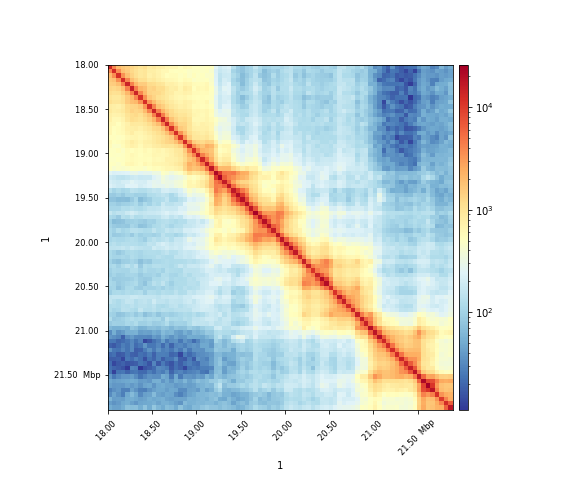
\includegraphics[scale=0.205, trim=50 45 50 30,clip]{c_50kb}}
    \subfloat[RUST]{           
    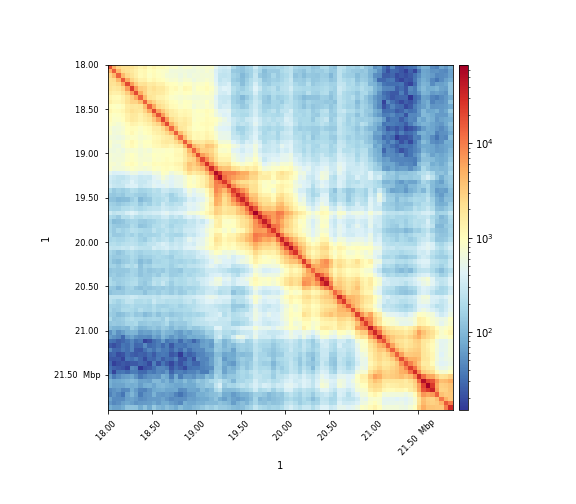
\includegraphics[scale=0.205, trim=50 45 50 30,clip]{c_rust_50kb}} \\
    \subfloat[KR]{             
    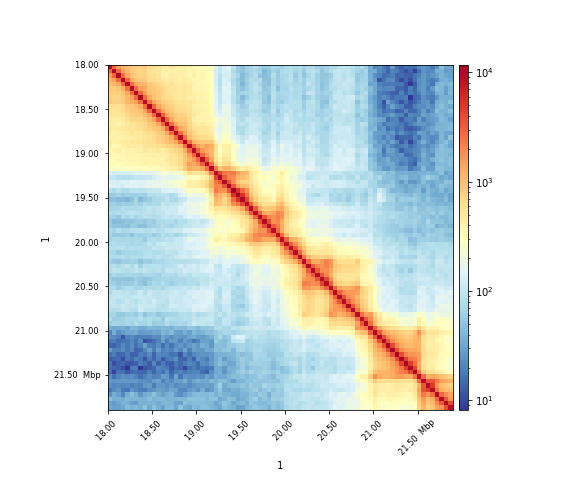
\includegraphics[scale=0.205, trim=50 45 50 30,clip]{c_kr_50kb}}
    \subfloat[ICE]{            
    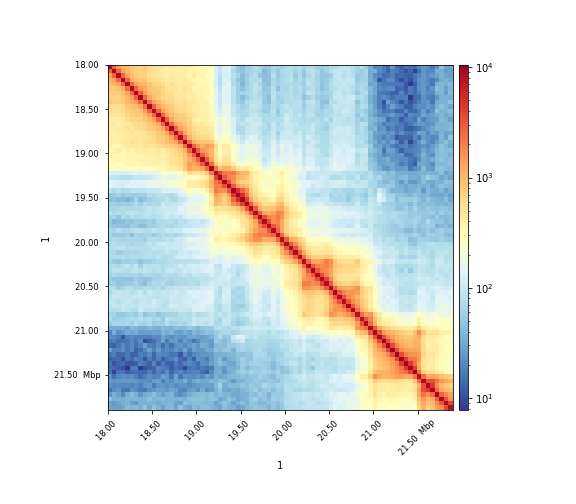
\includegraphics[scale=0.205, trim=50 45 50 30,clip]{c_ice_50kb}}
    \end{figure}
\end{frame}


\section{Conclusion}


\begin{frame}[c]{Conclusion Regarding the Integration of RUST}
    \begin{itemize}[<+(1)->]
        \item Test the alternatives more
        \item Better integration should be possible
        \item All in all: Went better than expected
    \end{itemize}
\end{frame}


\begin{frame}[c]{Conclusion Regarding Computation Comparisons}
    \begin{itemize}[<+(1)->]
        \item Reduction of memory usage during correction achieved
        \item Reduction of runtime achieved
        \item Parallelism does not offer significant benefits yet
    \end{itemize}
\end{frame}


\begin{frame}[c]{Remaining Questions}
    \begin{itemize}[<+(1)->]
        \item Writing code for faster parallelism
        \item Speedup when parallelizing more
        \item Pure implementations needing even less memory?
        \item Is KR faster for bigger matrices?
    \end{itemize}
\end{frame}





%%%%%%%%%%%%%%%%%%%%%%%%%%%%%%%%%%%%%%%%%%%%%%%%%%%%%%%%%%%%%%%%%%%%%%%%%%%%%%%%%%%%%%%%%%%%%%%%%%%



%%%%%%%%%%%%%%%%%%%%%%%%%%%%%%%%%%%%%%%%%%%%%%%%%%SOURCES%%%%%%%%%%%%%%%%%%%%%%%%%%%%%%%%%%%%%%%%%%
\section{Sources}
\setbeamertemplate{bibliography item}[triangle]
\begin{frame}[c, fragile, allowframebreaks]{Sources}
% \begin{frame}[c, allowframebreaks]{Sources}
% \bibliographystyle{plainnat}
% \bibliographystyle{plain}
\bibliographystyle{ieeetr}
\bibliography{references.bib}
\end{frame}


\appendix
\backupbegin

\begin{frame}[c]{Rust: Code Example}
    \begin{codeboxed}{Code Example 1}
    \inputminted[linenos, fontsize=\normalsize]{Rust}{code/code_ownership.rs}
    \end{codeboxed}
\end{frame}

\begin{frame}[c]{Rust: Code Example}
    \begin{codeboxed}{Output Nr. 1}
        \footnotesize
        \verbatiminput{code/output1.txt}
    \end{codeboxed}
\end{frame}

\begin{frame}[c]{Rust: Code Example}
    \begin{codeboxed}{Code Example 2}
    \inputminted[linenos, fontsize=\normalsize]{Rust}{code/code_ownership2.rs}
    \end{codeboxed}
\end{frame}

\begin{frame}[c]{Rust: Code Example}
    \begin{codeboxed}{Output Nr. 2}
        \footnotesize
        \verbatiminput{code/output2.txt}
    \end{codeboxed}
\end{frame}

\backupend


\end{document}
